\section*{Hardware Experiment}
To perform the Experiment, the First thing is the high-voltage 
generator, then the structure itself, and lastly measurements.
\subsection*{High voltage generation}
The circuit used was discussed in the previous section. Here the 
circuit in reality %Add reference to the figure using \ref{label}
%\begin{figure}[ht]
%	\centering
%	\includegraphics{}
%	\label{}
%\end{figure}
\subsection*{Hardware Measuring}
The Quantities to measure:
\begin{enumerate}
	\item Applied Voltage: we intend to measure it using simple
		voltage divider in fig.\ref{voltage_divider},
		the problem with this method is the loading effect, since 
		this is a high voltage of around 30kV in order to avoid this
		the effect very big resistors should be used, we use 7 resistor
		1M.
		\begin{figure}[ht]
			\centering
			\label{voltage_divider}
			% XCircuit output "Voltagedivider.tex" for LaTeX input from Voltagedivider.eps
\def\putbox#1#2#3#4{\makebox[0in][l]{\makebox[#1][l]{}\raisebox{\baselineskip}[0in][0in]{\raisebox{#2}[0in][0in]{\scalebox{#3}{#4}}}}}
\def\rightbox#1{\makebox[0in][r]{#1}}
\def\centbox#1{\makebox[0in]{#1}}
\def\topbox#1{\raisebox{-0.60\baselineskip}[0in][0in]{#1}}
\def\midbox#1{\raisebox{-0.20\baselineskip}[0in][0in]{#1}}
   \scalebox{0.5}{
   \normalsize
   \parbox{2.45312in}{
   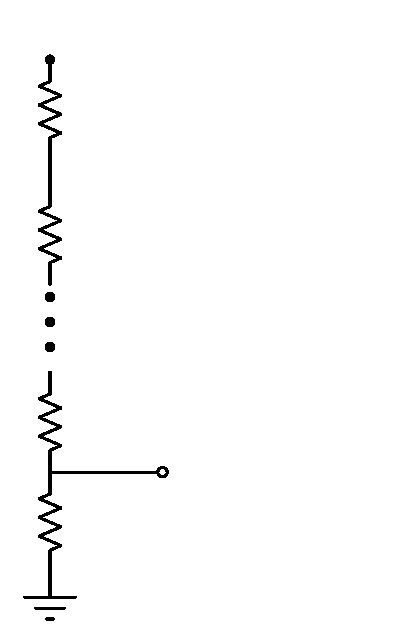
\includegraphics[scale=1]{images/Voltagedivider.eps}\\
   % translate x=208 y=444 scale 0.38
   \putbox{0.31in}{3.87in}{1.20}{$V_{applied}$}%
   \putbox{1.06in}{1.12in}{1.20}{$V_{meaured}$}%
   } % close 'parbox'
   } % close 'scalebox'
   \vspace{-\baselineskip} % this is not necessary, but looks better

			\caption{voltage divider to measure the applied
			voltage}
		\end{figure}
		
	\item Power dissipation: it could be measured 
		\begin{equation}
			P = V_{in} \times I_{in}
		\end{equation}
		where $V_{in}$ is the input voltage and $I_{in}$ is the 
		input  current

	\item Thrust/Lift: Due to a lack of fine equipment the following
		method is used, we load the ionocraft with some weight and 
		when the ionocraft reaches equilibrium the weight of the 
		ionocraft is measured using a sensitive scale.

	\item gap distance: since the gap distance measured in
		centimeters, it is safe to measure it using a regular ruler.
		
\end{enumerate}
\subsection*{Experiment Setup:}
\begin{enumerate}
	\item Setup 1:\\
	In Setup 1, we prepared a Triangular ionocraft with a side length
	10 cm, and aluminum foil height of 4cm,
	with wooden skewers as support.
	The voltage applied $\approx 30KV$ (we couldn't measure it
	accurately due to the loading effect, but the arc established at
	around 1cm).
	Unfortunately, the ionocraft didn't fly, the ionocraft was too
	heavy to take off, and the thrust was too weak.
	First, we try to increase the input voltage from 12 volts up
	to 19 volts, but unfortunately, the thrust was too weak to make
	the ionocraft fly, we couldn't measure the thrust of
	due to a lack of equipment and the ionocraft is still fixed.

\begin{figure}[ht]
	\centering
	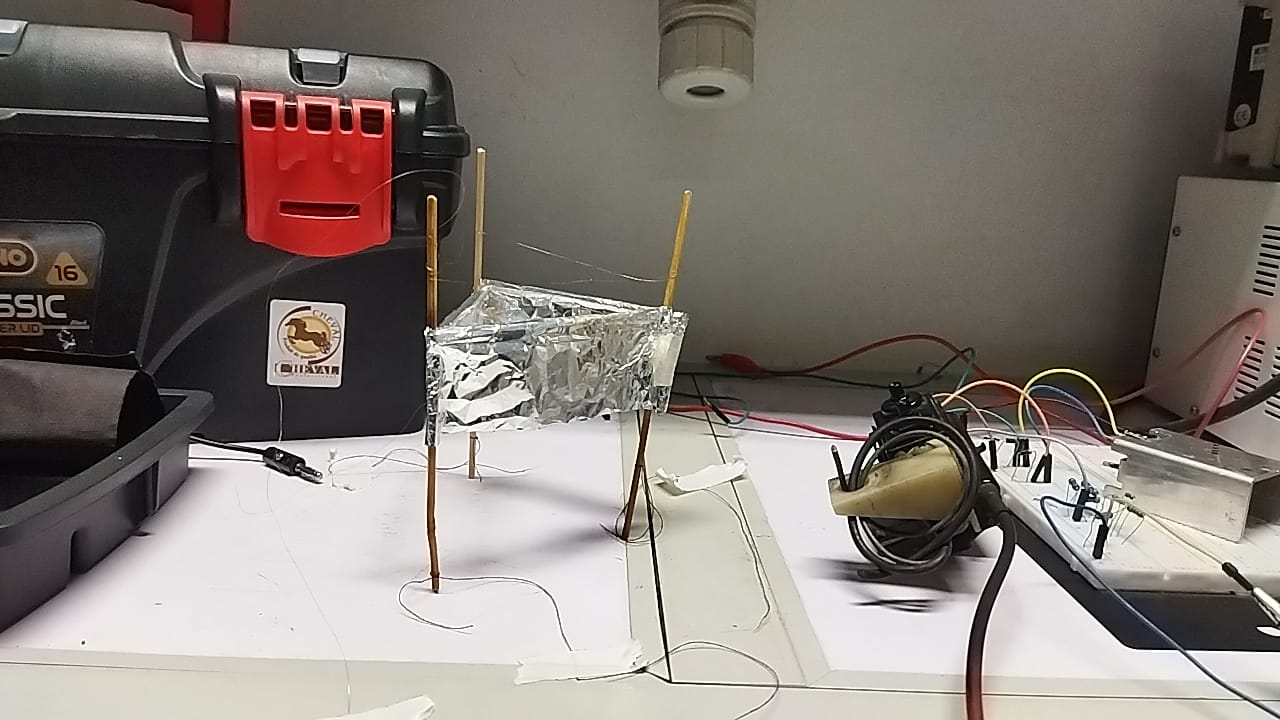
\includegraphics[scale=0.3]{images/results images/setup1.jpeg}
	\caption{Setup 1 Triangular ionocraft with wooden skewers
	support}
\end{figure}

	\item Setup 2:\\
	In this setup we made the following changes: the wooden
	skewers were replaced by plastic straws, the length
	of the support was reduced, and the height of the aluminum foil
	was reduced ( and unfortunately not measured), and third the input
	voltage was increased to 30 volts.\\
	Unfortunately, the ionocraft didn't fly, and the thrust was
	stronger(and again not measured as the ionocraft was standstill
	).
	\newpage
	Now, we may make changes to the circuit generating the High
	voltage itself, we plan to make the ionocraft lighter
	and the collector smoother
	or worst case change the structure itself.
	We should also change the measuring technique, to allow for
	measuring weak Lifts even when the ionocraft is on the ground.
	\begin{figure}[ht]
		\centering
		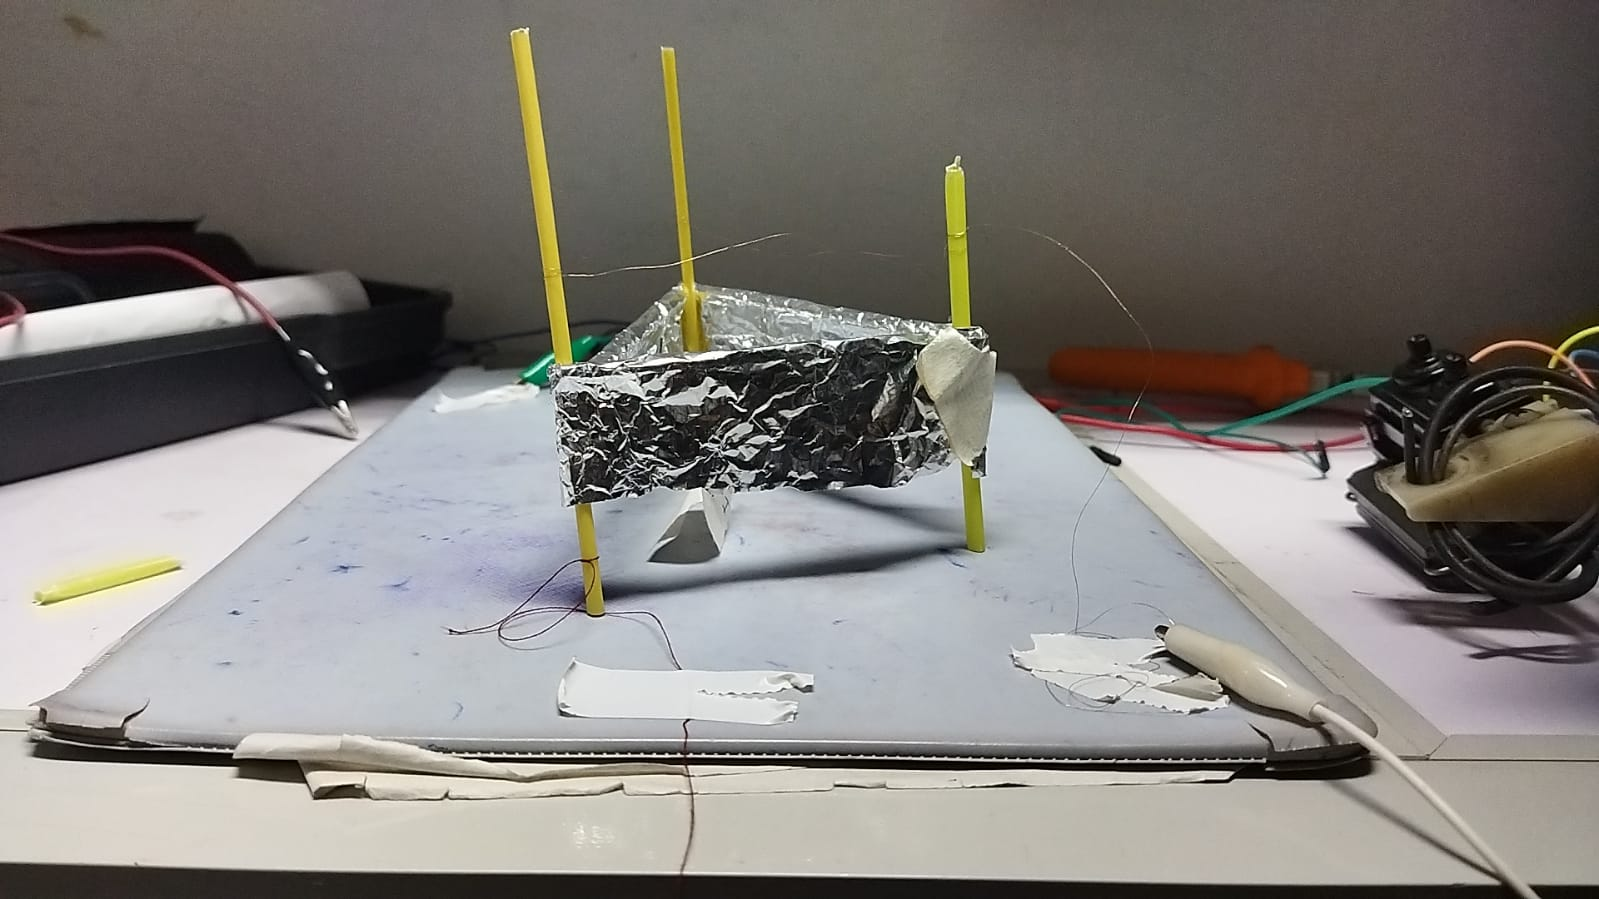
\includegraphics[scale =0.27]{images/results images/setup2.jpeg}
		\caption{Setup 2 Triangular ionocraft with plastic straws}
	\end{figure}

	For now, we will use another Experiment data to test the models.
\end{enumerate}


